% mn2esample.tex
%
% v2.1 released 22nd May 2002 (G. Hutton)
%
% The mnsample.tex file has been amended to highlight
% the proper use of LaTeX2e code with the class file
% and using natbib cross-referencing. These changes
% do not reflect the original paper by A. V. Raveendran.
%
% Previous versions of this sample document were
% compatible with the LaTeX 2.09 style file mn.sty
% v1.2 released 5th September 1994 (M. Reed)
% v1.1 released 18th July 1994
% v1.0 released 28th January 1994

%\documentclass[useAMS,usenatbib]{mn2e}
\documentclass[usenatbib]{mn2e}
%\documentclass[usenatbib,aas_macros]{mn2e}

% If your system does not have the AMS fonts version 2.0 installed, then
% remove the useAMS option.
%
% useAMS allows you to obtain upright Greek characters.
% e.g. \umu, \upi etc.  See the section on "Upright Greek characters" in
% this guide for further information.
%
% If you are using AMS 2.0 fonts, bold math letters/symbols are available
% at a larger range of sizes for NFSS release 1 and 2 (using \boldmath or
% preferably \bmath).
%
% The usenatbib command allows the use of Patrick Daly's natbib.sty for
% cross-referencing.
%
% If you wish to typeset the paper in Times font (if you do not have the
% PostScript Type 1 Computer Modern fonts you will need to do this to get
% smoother fonts in a PDF file) then uncomment the next line
% \usepackage{Times}

%%%%% AUTHORS - PLACE YOUR OWN MACROS HERE %%%%%

\usepackage{graphicx,graphics}
\usepackage{amsmath}
\usepackage{color}


\newcommand{\kms}{km\,s$^{-1}$}
\newcommand{\ncomets}{N_{\rm c}}
\newcommand{\ratio}{\mathcal{R}}
\newcommand{\lags}{\mathcal{L}_{\rm s}}
\newcommand{\lagc}{\mathcal{L}_{\rm c}}
\newcommand{\rvir}{r_{\rm vir}}
\newcommand{\qc}{Q_{\rm c}}
\newcommand{\qe}{Q_{\rm e}}
\newcommand{\qh}{Q_{\rm h}}
\newcommand{\nna}{N_{\rm 1}}
\newcommand{\nnb}{N_{\rm 2}}
\newcommand{\nnc}{N_{\rm 3}}
\newcommand{\nb}{\texttt{NBODY6++GPU}}
\newcommand{\msun}{M_\odot}

%%%%%%%%%%%%%%%%%%%%%%%%%%%%%%%%%%%%%%%%%%%%%%%%%%%%%%%%%%%%%%%%%%%%%%%%%%

\title[Comets in star clusters: I. Dynamics of free-floating comets]{Comets in star clusters: I. Dynamics of free-floating comets}  

\author[Qi Shu et al.]{Qi Shu$^{1,2}$\thanks{E-mail:shuqi@pku.edu.cn}, M.B.N. Kouwenhoven$^{4}$, Rainer Spurzem$^{1,3,5}$\\
  $^{1}$Kavli Institute for Astronomy and Astrophysics, Peking University, Yiheyuan Lu 5, Haidian Qu, 100871, Beijing, China\\
  $^{2}$Department of Astronomy, School of Physics, Peking University, Yiheyuan Lu 5, Haidian Qu, 100871, Beijing, China\\
  $^{3}$National Astronomical Observatories and Key Laboratory of Computational Astrophysics, Chinese Academy of Sciences, \\
  20A Datun Rd., Chaoyang District, 100012, Beijing, China\\ 
  $^{4}$Department of Mathematical Sciences, Xi'an Jiaotong-Liverpool University, 111 Ren'ai Road, \\
  Suzhou Dushu Lake Science and Education Innovation District, Suzhou Industrial Park, Suzhou 215123, P.R. China \\
  $^{5}$Astronomisches Rechen-Institut, Zentrum f\"ur Astronomie, University of Heidelberg, M\"onchhofstrasse 12-14, \\
69120, Heidelberg, Germany \\
}

\begin{document}

\date{Accepted 2017 XX X. Received 2017 XX X; in original form 2017 XX X}

\volume{XXX} \pagerange{XXXX-XXXX} \pubyear{2017}

\maketitle

\label{firstpage}

\begin{abstract}
The Sun's Oort Cloud contains trillions of comets in weakly bound, highly eccentric orbits. Most stars are formed in star clusters, where comets are easily removed from their host stars. We carry out numerical simulations to investigate the dynamical evolution of comet populations in star clusters.


\end{abstract}

\begin{keywords}
minor planets, asteroids: general -- planetary systems -- planet-disc interactions -- methods: numerical -- planets and satellites: dynamical evolution and stability -- protoplanetary discs
\end{keywords}

\section{Introduction}

%%origion of comets in solar system
The outer Oort Cloud in our Solar system contains roughly $5 \times10^{11}$ comets with absolute magnitudes $H < 17$ \citep{Francis:2005aa}. These comets are thought to have originated during the planet formation process, when many planetesimals collided with the newly-formed planets and the Sun, but many others got ejected to the outer fringes of the Solar system. Some obtained a velocity beyond the local escape velocity and became free-floating comets in the Galactic field, while others obtained highly-eccentric orbits in the Oort cloud. Given the ubiquity of exoplanets in the Galactic field, it is not unreasonable that a similar process has also occurred during the formation of other stars, and that our Galaxy is filled with Oort clouds and free-floating comets. In fact, several authors claimed to have found evidence for so-called exocomets in system such as $\beta$~Pictoris \citep[e.g.,][and references therein]{Welsh:2016aa} and KIC~8462852 \citep[e.g.,][and references therein]{Bodman:2016aa, Boyajian:2016aa}

%%invitation to study comets in star cluster
The vast majority of young stars are found in or near star forming regions that contain hundreds to millions of stars. These star forming regions either disperse within several tens of millions of years, while others remain bound and become the open clusters and globular clusters that we know today \citep[e.g.,][]{de-Grijs:2007aa}. Isotope studies of meteorites even suggest that our own Sun was once part of a star cluster that has long dispersed. Given that most stars are formed in crowded stellar environment, it is worthwhile to investigate what happens to the comet populations belonging to stars in these environments. 

%% origin od free-floating comets
During the planet formation process, a large number of comets is ejected from their host star systems after scattering events with (proto-)planets. In a star cluster environment, close encounters between comet-hosting stars and other cluster members can also result in the ejection of comets. These two processes are responsible for the injection of large numbers of comets into the star cluster \citep[e.g.,][]{Brasser:2015aa}. These comets remain part of the star clusters until they escape from the cluster through ejection or evaporation. In some cases, these comets may be captured by other stars in or near the cluster. The balance between the injection and escape of comets into/from the cluster determines the total number of free-floating comets at a certain time in a star cluster. 

%%Mention panspermia to be added

%%observation of ffc in solar system
All presently-known comets come almost certainly from the outskirts of our solar system \citep{Dones:2015aa}. The most likely interstellar comet (i.e., a comet originating from outside our solar system is C/2007~W1 (Boattini), which has a derived velocity-at-infinity of 0.2~\kms{} \citep{Dybczynski:2015aa}. However, given that the velocity dispersion in the Galactic field is two orders of magnitude larger than this value, the reconstructed orbit of C/2007~W1 is more likely the result of gravitational perturbations by other bodies. Moreover, due to the large velocity dispersion in the Galactic field, our Solar system is unlikely to capture free-floating comets from the field. Currently, Comet 96P/Machholz is the best candidate for comets with interstellar origin, (Schleicher 2008) because of its high eccentricity and inclination as well as different composition than other comets.

%%comets in star cluster

The situation is different in star cluster. In star clusters, many comets are expected to be liberated from their host star. The origin of free-floating comets is two-fold: (1) comets that are ejected from their host star systems, for example as a result of a dynamical interaction with planet, and (2) comets that are removed from their host star following a close encounter with another star cluster member. In the clusters, all stars and most free-floating comets ejected from their host stars have similar velocities. As a result, free-floating comets can remain bound to the star cluster for many dynamical times, and the capture probabilities are non-negligible.

Star cluster members occasionally pair up and form new binary systems. Such newly-formed systems are often transient \citep[e.g.,][]{Moeckel:2011aa}, but several several may survive for much longer times, in particular when they remain in the outskirts of the star cluster or when they have escaped \citep{Kouwenhoven:2010aa}. Free-floating planets are also captured \citep{Perets:2012aa}, which is particular interest to us, as our free-floating comets can be considered as test particles. Unlike multi-planet systems, multi-comet systems do not suffer from strong scattering effects. Re-captured multi-comet systems can thus survive for long periods of time in star clusters.

%% simulations

\cite{Spurzem:2009aa} investigated the instabilities of planetary systems in star clusters, and the ejection process of planets from their host system.  \cite{Wang:2015ab}  studied the survival rate of these ejected free-floating planets (FFPs). In this paper, We will consider both the recaptured FFPs and planets ejected out of star cluster.

This article is organised as follows. In \S\ref{section:method} we describe our numerical method and initial conditions. We discuss the evolution of the star clusters and the free-floating comet populations in \S\ref{section:results}. Finally, we summarise our results and discuss the implications of our findings in \S\ref{section:conclusions}.

\section{Methodology and initial conditions} \label{section:method}


\subsection{Numerical method}

Simulations are run using a version of \nb\ \citep{Wang:2015ab} that is adjusted to suit the purpose of our simulations. Stellar evolution and binary evolution are implemented following the prescriptions of Cambridge stellar evolution package \citep{Eggleton:1989aa, Hurley:2000aa}.

We have adjusted the \nb\ package to be able to integrate large numbers of comets. The mass of comets is many orders of magnitude smaller than that of stars, and the comets can therefore be safely treated as test particles. Star-comet binaries are excluded from KS scheme. When calculated the gravitational interaction from other particles to a certain star, comets are ignored. Also, we disabled the stellar evolution of comets. %\textbf{GPU part to be discussed.}
As comets can be safely treated as massless particles, the choice for total number of comets, $\ncomets$ will not affect our results, other than statistically. The results can be easily scaled up to realistic values of $\ncomets$. 
All particles (stars, comets, or multiple systems) are considered as bound to the star clusters when they are within two tidal radii of the cluster centre. Otherwise, they are considered to have escaped from the star cluster.

Binary systems, which can be either star-star or star-comet systems. We do not consider comet-comet binaries, as these do not occur when considering massless particles. For each pair of bodies in the system we mutual binding energy. If this mutual binding energy is negative (i.e., we have identified a candidate binary), we proceed as follows: (1) if both bodies have mass, then they only form a bound binary if they are each other's mutual nearest neighbours with mass;, and (2) if only one body has mass, then the two bodies only form a binary if the body with mass is the nearest body with mass of the massless particle. We then obtain the orbital elements of each binary. We consider only binaries with semi-major axes less than ~ 1pc, which corresponds to the stability limit in the Galactic field. Note that one star can have multiple comet companions. Also, binary stars can have one or more comet companions in S-formation or P-formation.

\begin{figure}
  \centering
  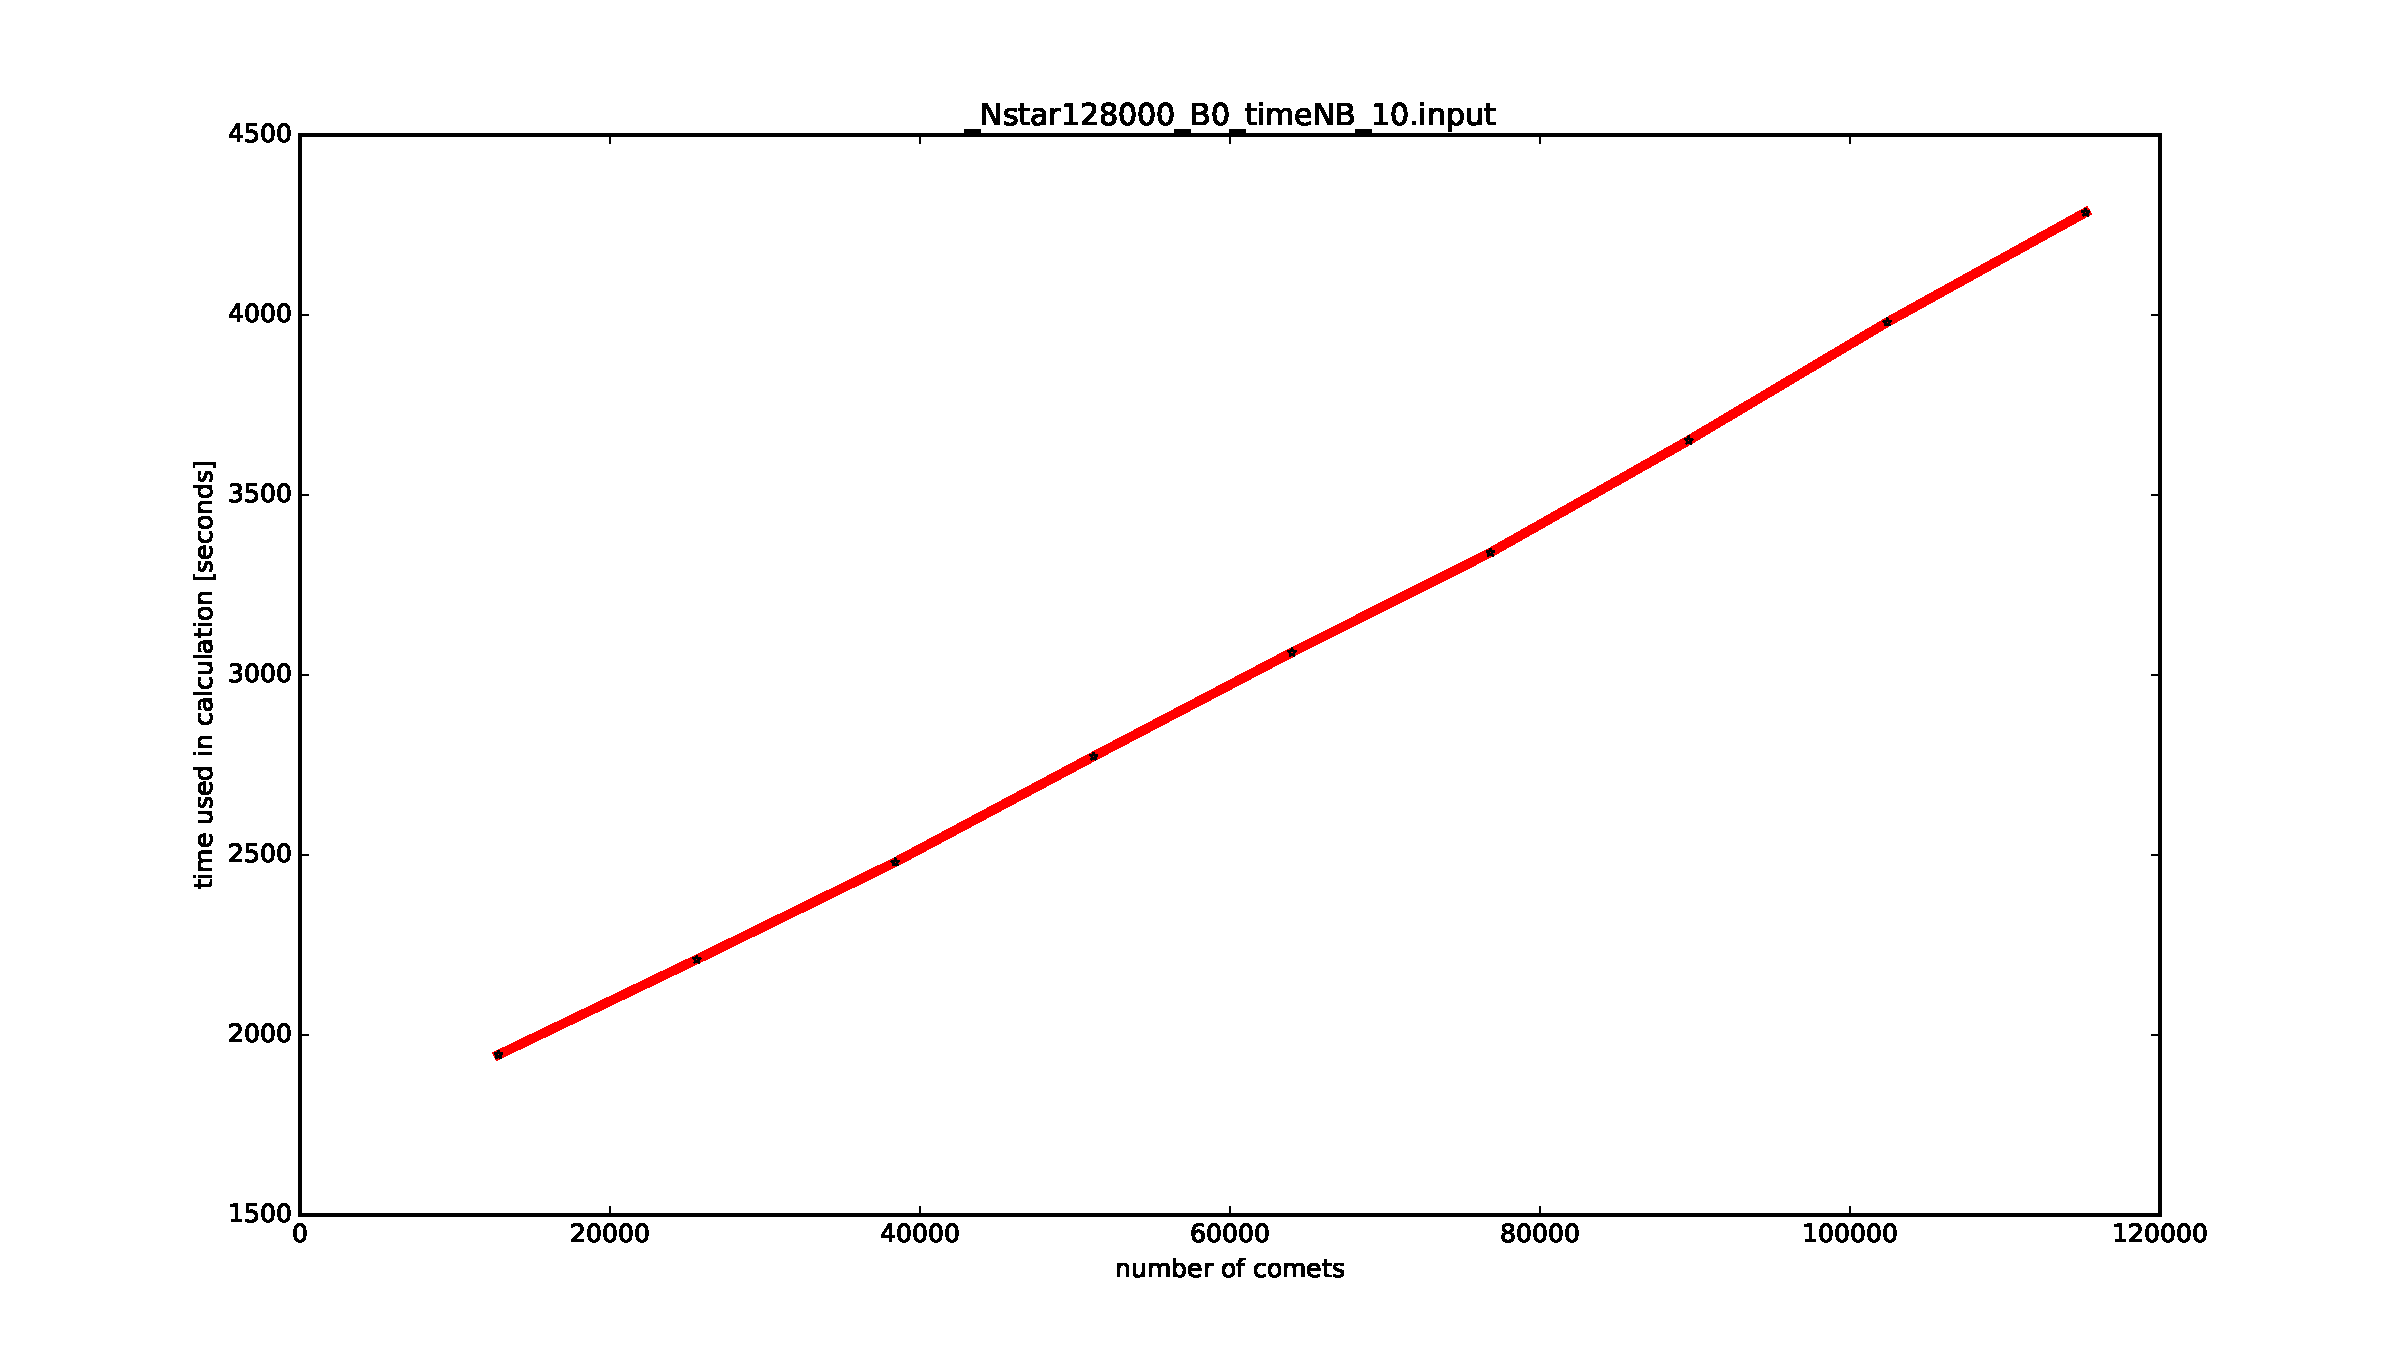
\includegraphics[width=0.5\textwidth,height=!]{time_used.pdf}
  \caption{Time used in simulations with same number of single star 128k, but different number of free-floating comets from 12.8k to 128k.}
  \label{fig:time_used}
\end{figure}

Comparing with the code used in \citep{Wang:2015ab}, the new code has better performance when more massless particles is added. Because we disable the interaction between massless particle, the time consuming is roughly $\alpha N_{star}^{2}+\beta N_{comet} N_{star}$, if we fix $N_{star}$, time consuming increased linearly with $N_{comet}$. The real simulation time used is shown as Figure \ref{fig:time_used}.


Our simulations are carried out on a workstation with an Intel CPU (i7-5960X CPU @ 3.00GHz) and two NVIDA GPU cards (GeForce GTX 980 Ti).

\subsection{Initial conditions}

\begin{figure}
  \centering
  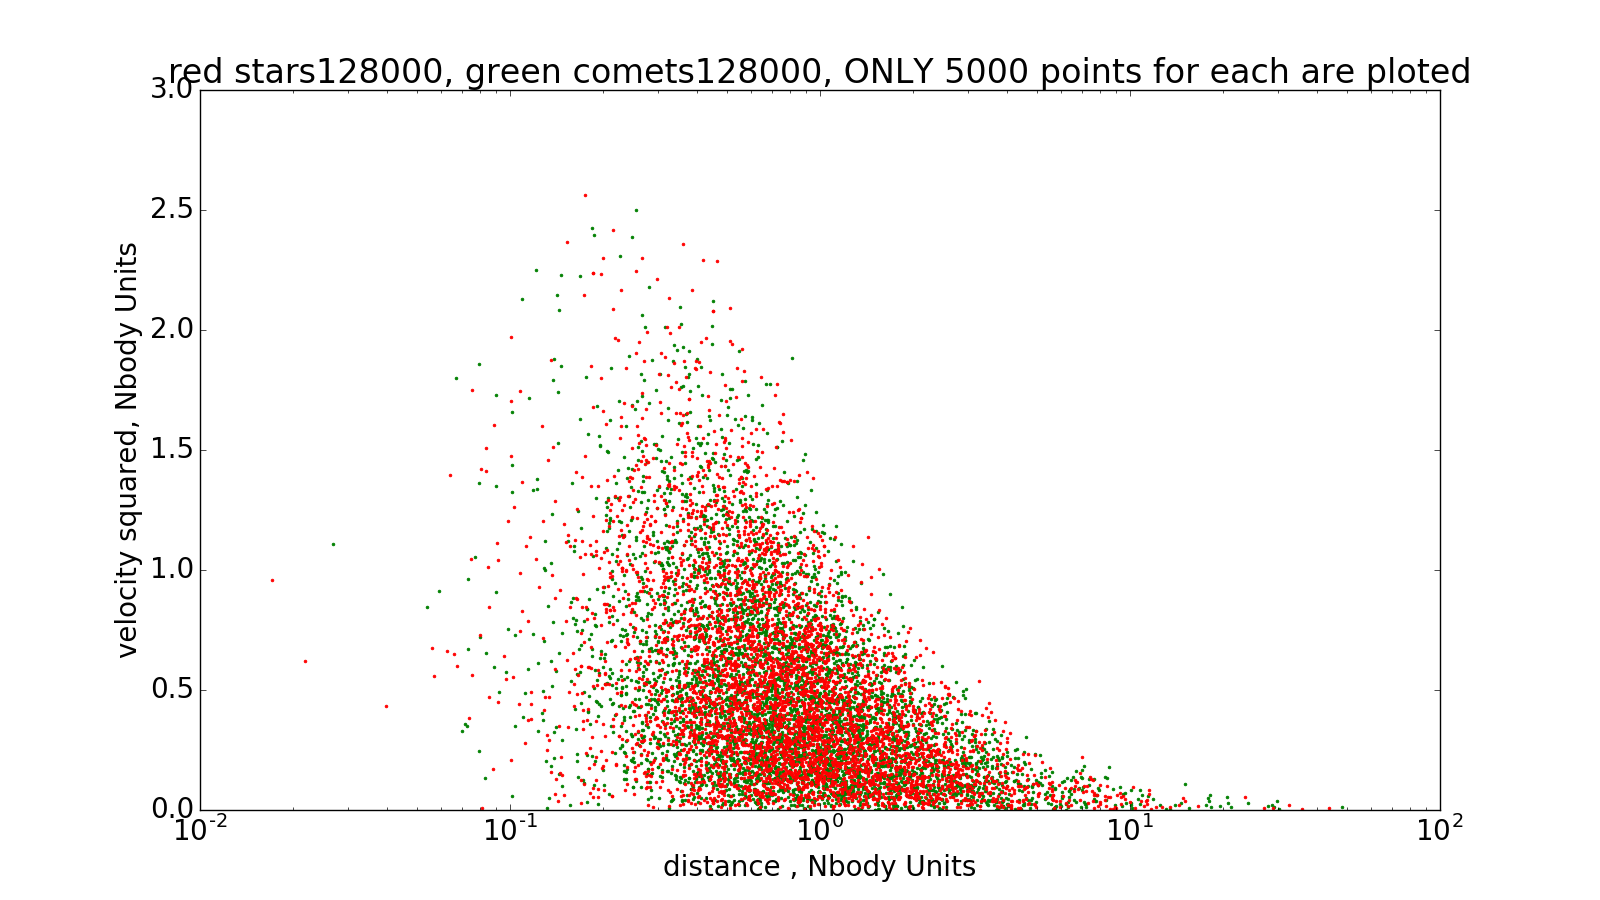
\includegraphics[width=0.5\textwidth,height=!]{v2_r.png}
  \caption{The velocity and distance distribution of particle in the simulation, $N_{star} = N_{comet} = 128k$, Q = 0.5.}
  \label{fig:v2_r}
\end{figure}

We evolve star cluster models that correspond to large open clusters or small globular clusters. Our initial conditions are summarised in Table~\ref{table:initial}. The positions and velocities of all stars are drawn from the \cite{Plummer:1911aa} model in virial equilibrium with a virial radius of $\rvir=5 \sim 20$~pc. Stellar masses are drawn from the Kroupa (2001) initial mass function (IMF) in the range $0.08-20\msun$. We do not include primordial binaries, nor do we include primordial mass segregation. One of the $v^{2} \sim r$ plots can be seen in Figure \ref{fig:v2_r}. Each model is embedded in a standard solar neighbour tidal field, see Table~\ref{table:tidal}.

\begin{table*}
\caption{Initial conditions for our default model.  \label{table:initial}}
\begin{tabular}{ll}
\hline
\hline
Quantity & Value \\
\hline
Number of stars & $ \nna  \sim 12.8k $ large open cluster \\
 & $\nnc  128k$  small globular cluster \\


Stellar IMF &  Kroupa(2001), extended to Brown Dwarf regime\\ %KZ(20) = 6 
Virial radius & $\rvir=20$~pc (probably following a mass-radius relationship) \\
Dynamical model & \cite{Plummer:1911aa} \\
Stellar evolution &  Enable mass loss \\ %P.P. Eggleton, M.J. Fitchett \& C.A. Tout (1989) Ap.J. 347, 998.
Tidal field & no tidal force\\ %KZ(14) = 0 
\hline
Comet mass & Test particles \\
Comet-to-star-ratio & $\ratio=\ncomets/N= 1$ \\
Comet spatial distribution & Statistically identical to stars \\
Comet velocity distributions & $\qe=0.5$ (in virial equilibrium with stars) \\
	& $\qc=0.9$ (hot) \\
\hline
\hline
\end{tabular}
\end{table*}

%%%%%%%%%%%%%%%%%%%%%%%%%%%%%%%%%%%%%%%%%%%%%%%%%%%%

\begin{table*}
\caption{standard solar neighbour tidal field \label{table:tidal}}
\begin{tabular}{ll}
\hline
\hline
POINT-MASS MODEL (NB unit) \\
\hline
  MG  & $1.5 \times 10^8$  \\
  RG  &  $7.8 \times 10^3$  \\
  OMEGA & $1.8 \times 10^{-2}$ \\
  RTIDE & $11.5$  \\
  RBAR & $1.09$ \\
\hline
DISK MODEL \\
\hline
    MD &  $8.1 \times10^7$  \\
    A &  $3.7 \times10^3$  \\
    B &  $4.6 \times10^2$\\
\hline
SCALED ORBIT\\
\hline
    RG &  $7.78 \times 10^3$,  0.00,  0.00  \\
    VG &   0.00,  $1.41 \times10^2$,  0.00  \\
    $V_{0}$ &   $0.00$\\
\hline
\hline
\end{tabular}
\end{table*}



The population of $\ncomets$ free-floating planets is constructed independently of that of the stars. Their positions are also drawn from the \cite{Plummer:1911aa} model with a virial radius identical to that of the stellar mass distribution. Their velocity distribution is also constructed from the \cite{Plummer:1911aa} model, with a different $Q$ than the stars in order to investigate the evolution of different systems. We investigate the evolution of comet populations in different virial states:  $\qe=0.5$ (in equilibrium with the stellar population), and $\qh=0.9$ (hot). We did not discuss the case of $Q < 0.5$ because when comets are liberated from their host stars (through ejection or external perturbations), their kinetic energy is beyond the stars's escape velocity, and the comet population is therefore expected to be somewhat hotter than the stellar population. The models with $\qe$ represent comet ejections with negligible escape velocities, while the $\qh$ models represent high-velocity comet escapers.

Each model is integrated for 1000 $N$-body time units, corresponds to roughly 250 and 78.6 Myr. 

%%%%%%% maybe useful
%The crossing time is defined by $t_{cr} = 2R_{V}/\sigma$, where $R_{V}$ is virial radius obtained from $R_{V}=GM^{2}_{tot}/2|U|$ and $\sigma$ is the velocity dispersion ${\sigma}^{2} \simeq GM_{tot}/2R_{V}$
%%%%%%%%


\section{Numerical results}\label{section:results}

\subsection{Star cluster evolution}

Star cluster evolution is dominated by its stellar contents. For our model  $\nna$ and $\nnc$ star clusters, the initial crossing time are 0.93 and 0.22 Myr, respectively.

\begin{figure}
  \centering
  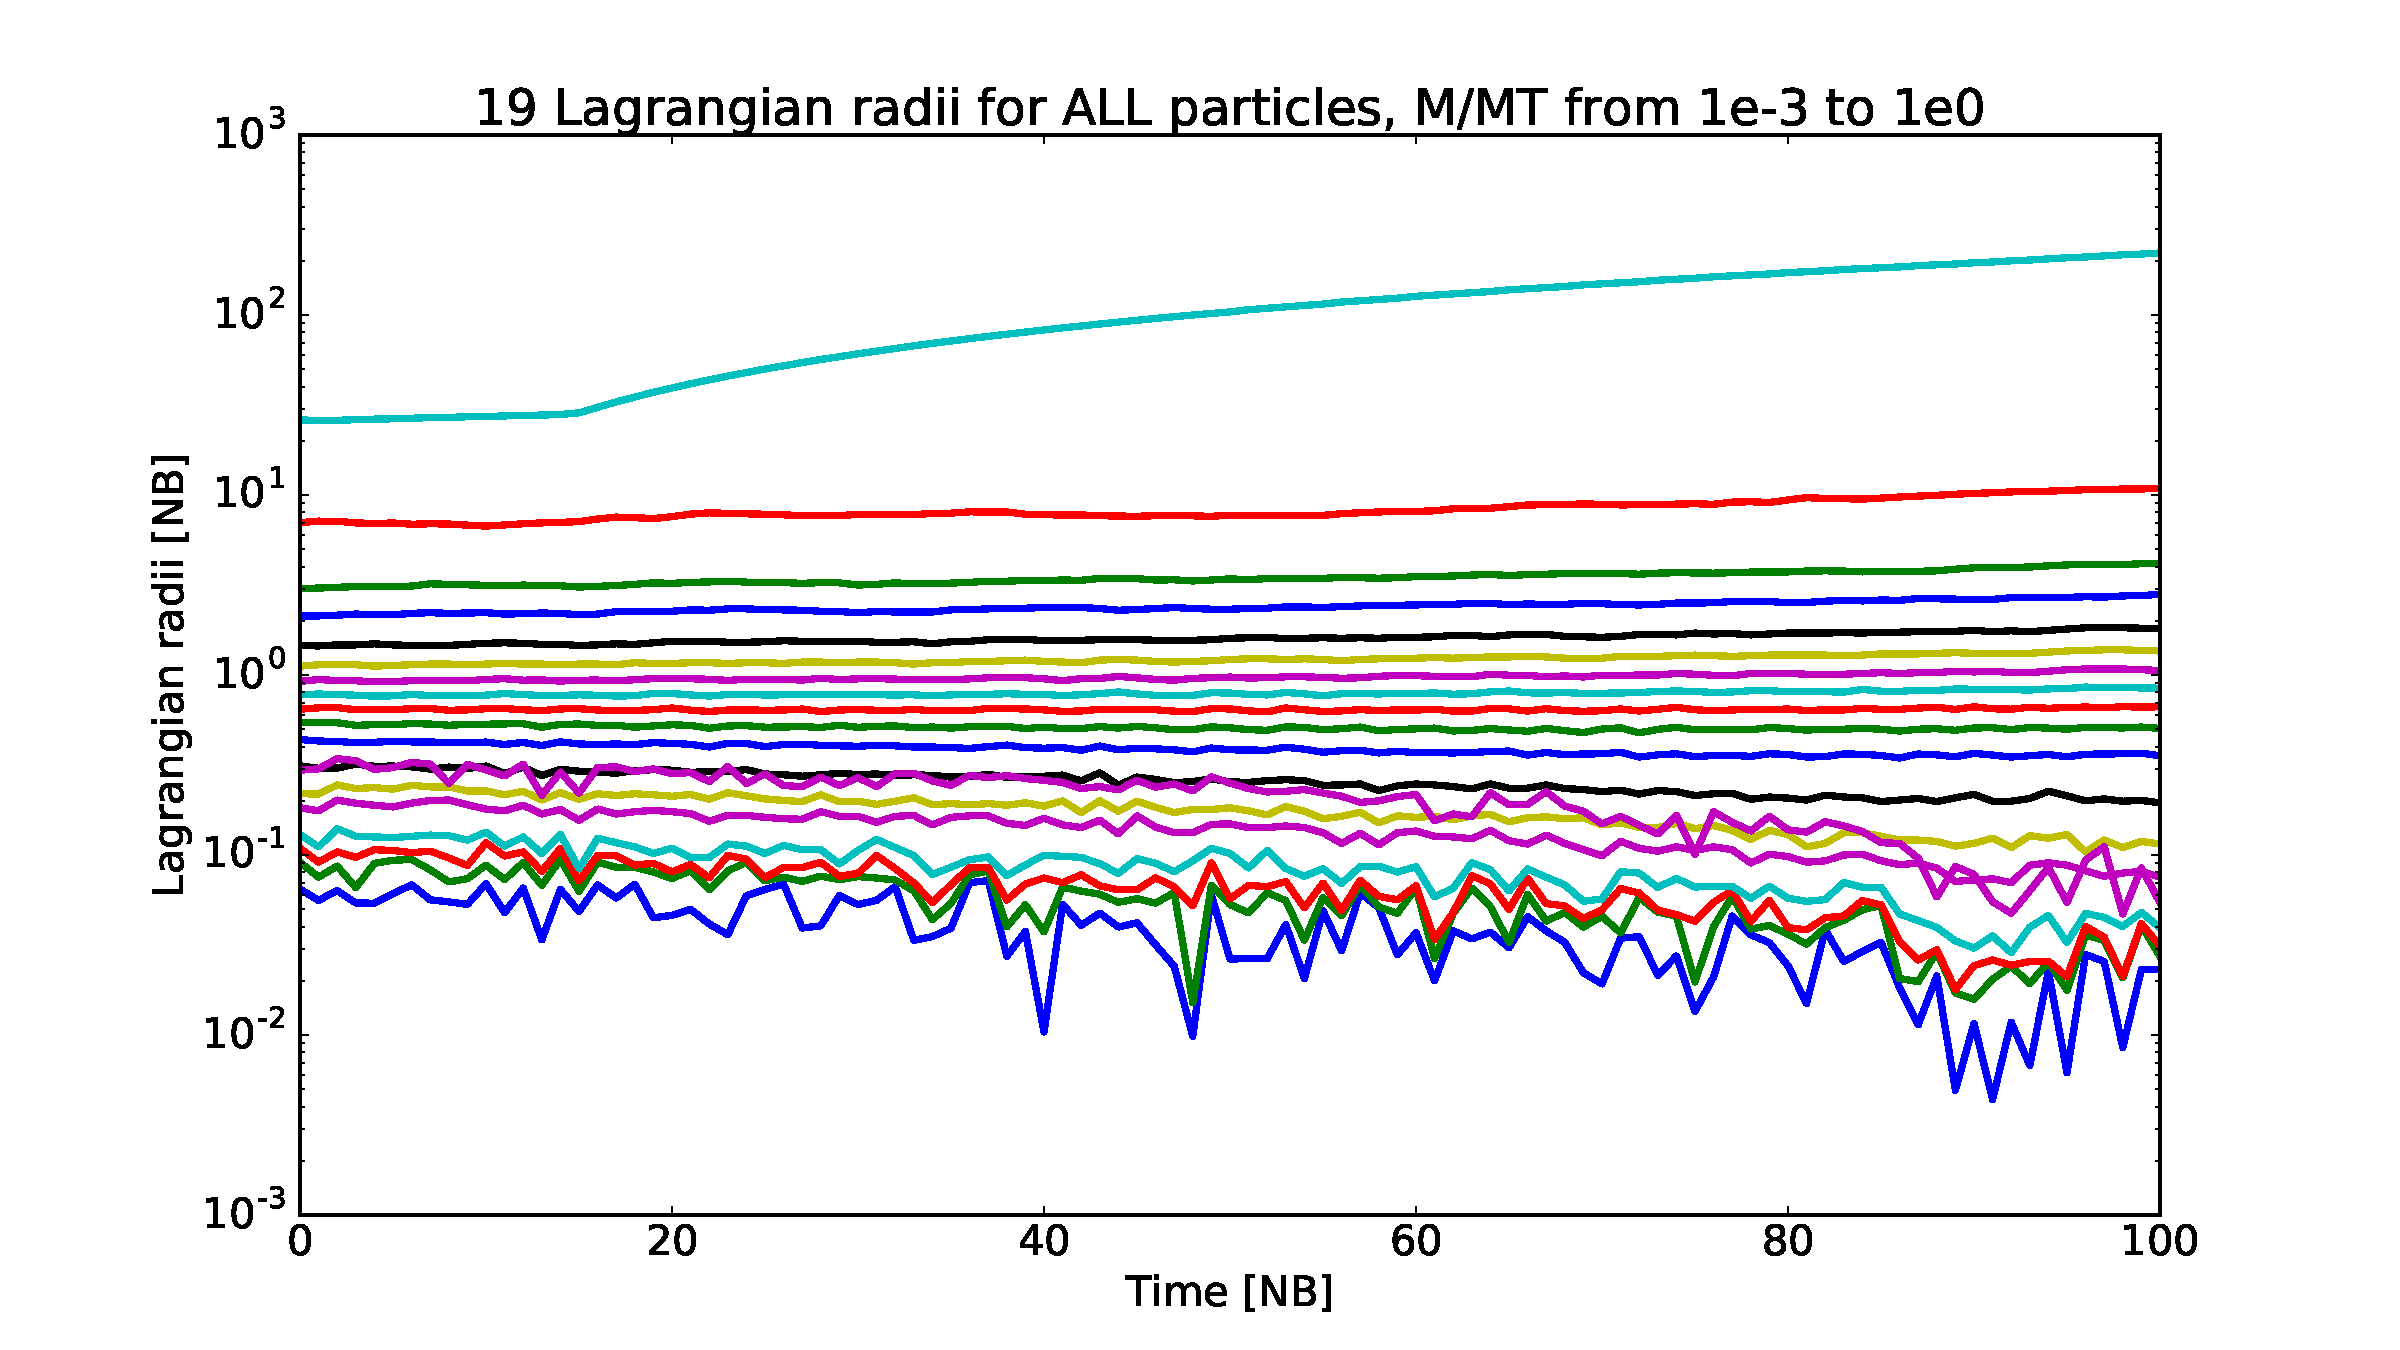
\includegraphics[width=0.5\textwidth,height=!]{lagrALL.pdf}
  \caption{Lagrangian radii for all particles, considering the tiny small mass of massless particles, it is also Lagrangian radii for all stars.}
  \label{fig:lagrALL}
\end{figure}

\begin{figure}
  \centering
  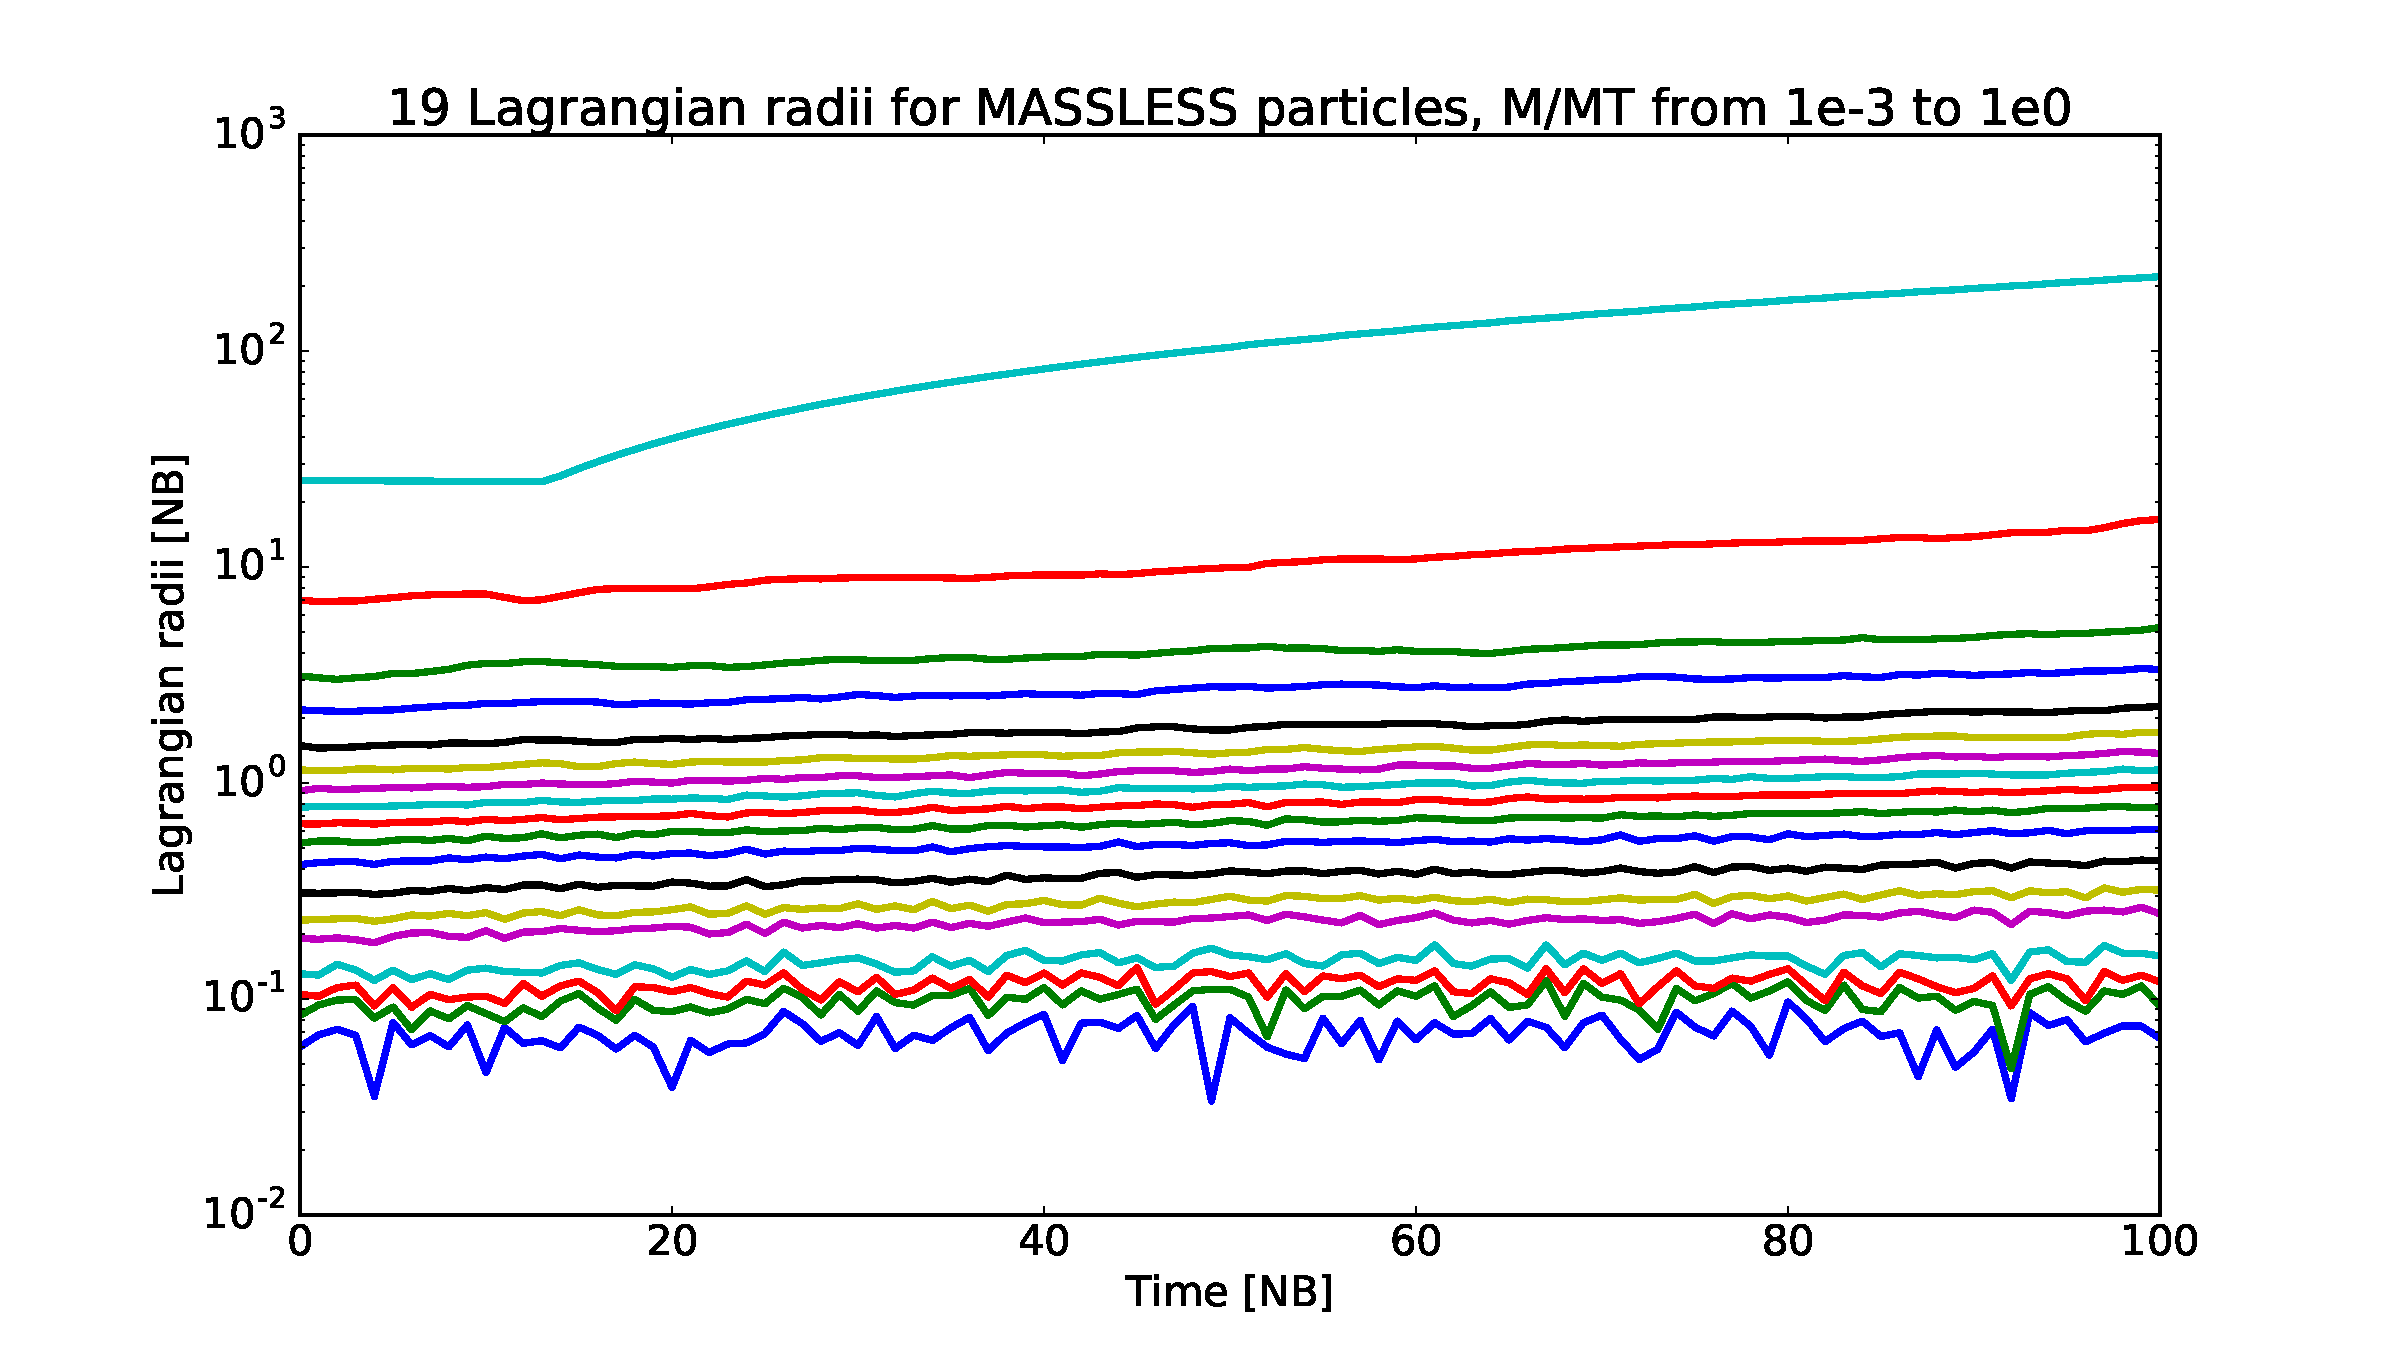
\includegraphics[width=0.5\textwidth,height=!]{lagrMASSLESS.pdf}
  \caption{Lagrangian radii for all massless particles.}
  \label{fig:lagrMASSLESS}
\end{figure}

We calculate the time-dependent Lagrangian radii for both the stellar population, $\lags(t)$ and for the cometary population $\lagc(t)$, see figure \ref{fig:lagrALL} and figure \ref{fig:lagrMASSLESS}.



Discuss evolution of the comet population here. Lagrangian radii, number of comets escaping, escape rates, comet-to-star ratios. Refer to \cite{Wang:2015ab}.

The stability of such star-comet systems is a strong function of the orbital semi-major axis \citep[e.g.,][]{Zheng:2015aa}.

\subsection{Re-capture of comets}

\begin{figure}
  \centering
  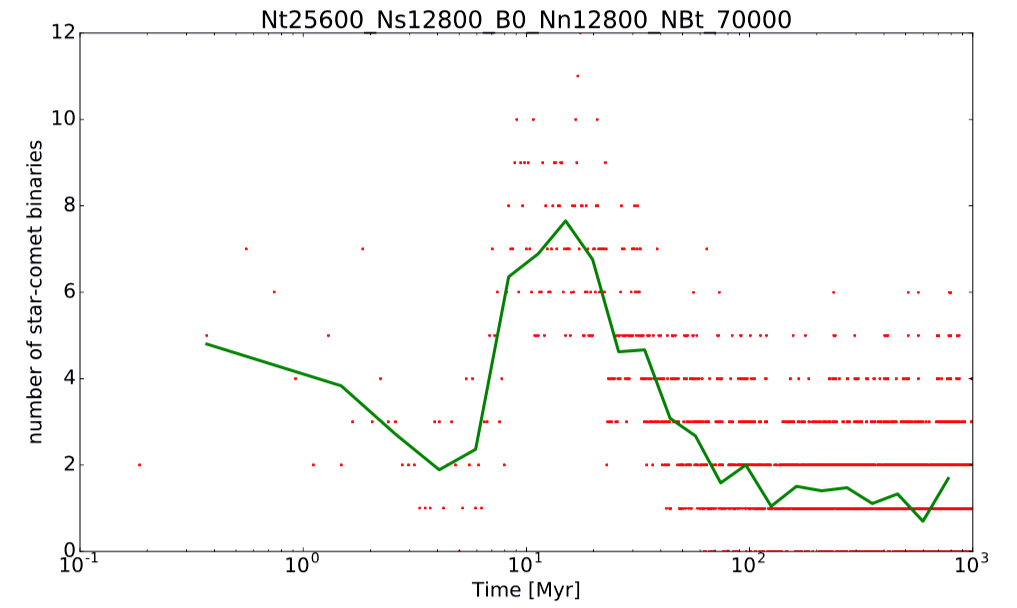
\includegraphics[width=0.5\textwidth,height=!]{Ns_c.png}
  \caption{Number evolution of star-comet binaries. The simulation starts with 128k single stars and 128k free-floating comets.}
  \label{fig:Ns_c}
\end{figure}

\textbf{NOTE: we do not have enough captured comets to give statistical results for this section}
While most free-floating comets escape, a small fraction is captured by stars. Describe how this fraction depends on time and on the other initial properties of the star cluster. Discuss the lifetime of such a captured object, and relate to escaping star-comet systems.

Orbital parameter discussions here. Semi-major axis distributions are possibly log-normal or possibly log-flat. The distribution is probably bi-model: smaller-$a$ and larger-$a$. The ones with smaller $a$ are the results of three-body interactions in star clusters. The ones with larger $a$ are all escapers, and they are formed from a capture process during their escape.

Eccentricity distributions. The eccentricity distributions will likely resemble the thermal eccentricity distribution, $f(e)=2e$ for $0\leq e < 1$ \citep{heggie:1975aa}. Equation descriptions for these: probably power laws with upper and lower limits. Correlations between semi-major axis and eccentricity distributions, possibly with a two-dimensional distribution function. 

A test simulation with our new code shows the result as figure \ref{fig:Ns_c}. 
%Discuss perihelion distributions, to check how they might interact with existing planetary systems.

%Discuss aphelion distributions, as these are probably more constrained by dynamical interactions than the semi-major axis distributions.


\subsection{Exchange of cometary material}

\textbf{NOTE: $X_{L}$ is mush smaller than $1\%$}

In this section we make analytical estimates for the level at which comets are exchanged between stars in a star cluster. Let $N_S$ be the number of stars in a star cluster, and $N_C$ be the average number of comets orbiting each star. Suppose also that each star loses a fraction $x_L$ of its comets, either through ejection or as a result of external perturbations. The total number of liberated comets in the cluster is then $x_LN_SN_C$. Suppose a fraction $x_R$ is of these free-floating comets is recaptured. Then the total number of recaptured comets is $x_Rx_LN_SN_C$, and each star captures $x_Rx_LN_C$ comets on average. This includes stars that remain bound to the cluster and stars that escape into the Galactic field. On average, the fraction of re-captured comets per star (relative to the remaining comets orbiting that star) is then $x_Rx_L(1-x_L)^{-1}$, which approximates to $x_Rx_L$ when $x_L\ll 1$. 

Suppose that each star loses $x_R=10\%$ of its comets, and that $x_L=1\%$ of the comets are re-captured. Then, on average, $0.1\%$ of the comets orbiting each star is foreign. When applying this simple model to our solar system, and use $N_C=10^{11}$, the total number of re-captured comets is of order a billion.

This simplistic calculation is merely an approximation, as we have ignored the dependence of $x_L$ and $x_R$ on the star cluster environment and on time, and also the dependence of $x_L$ on the architecture of the planetary system.

\section{Conclusions}\label{section:conclusions}

Summary of the project. Context, why we do it, what we do, how we do it. We find that 
%
\begin{itemize}
\item Comet escape rates and general dependence on initial conditions.
\item Comet capture rates
\item Orbital parameter distributions of captured comets
\item We predict that typically 0.1\% of the comets in our Solar system and in Oort clouds of other stars are re-captured, and have their origin in other planetary systems.

Future works.


In this work we have considered the dynamical evolution of comets in star clusters after these comets have been ejected from their host systems. In our next paper (Shu et al., in prep.) we will study the more realistic situation in which planets are initialised on circumstellar orbits. These simulations will naturally account for the release of comets from their host systems at appropriate times, appropriate positions in the star cluster, and with realistic ejection velocities. 

We have also ignored the presence of planetary companions. Although modelling of multi-planet systems is difficult \citep[][]{Hao:2013aa, Shara:2016aa}, it is possible in the AMUSE software environment \citep[see][]{Portegies-Zwart:2013aa, Pelupessy:2013aa, Cai:2016aa} or by sequentially integrating the stellar and planetary components \citep[][]{Cai:2015aa}. Moreover, it is a necessary step for obtaining a full understanding of comet populations in star clusters, in particular for understanding the transfer of material between planetary systems through comet-planet collisions. 

\end{itemize}

\section*{Acknowledgments}
We are grateful to Long Wang for his support during the initial phase of this project.
M.B.N.K. was supported by the Peter and Patricia Gruber Foundation through the PPGF fellowship, by the Peking University One Hundred Talent Fund (985), and by the National Natural Science Foundation of China (grants 11010237, 11050110414, 11173004 and 11573004). 
This publication was made possible through the support of a grant from 
the John Templeton Foundation and National Astronomical Observatories of the
Chinese Academy of Sciences. 
We acknowledge support by Chinese Academy of Sciences through the Silk Road
Project at NAOC, through the Chinese Academy of Sciences Visiting Professorship for Senior International Scientists, Grant Number 2009S1-5 (R.S.), and through the "Qianren" special foreign experts program of China.
The special GPU accelerated supercomputer {\tt laohu} at the Center of Information and
Computing at National Astronomical Observatories, Chinese Academy of Sciences, funded by Ministry of Finance of People's Republic of China under the grant ZDY Z2008-2, has been used for some simulations. 




%****************************************************************************%

%-------------------------------------------------------------------
%   bibliography
%-------------------------------------------------------------------
\clearpage
\phantomsection
\bibliographystyle{apj} 
\bibliography{Qi} 

%\begin{thebibliography}{999}
%\begin{thebibliography}{999}


\end{document}

